\section{Christensen-Burley BSSRDF profile importance sampling}
\label{section:burley_importance}
Importance sampling of the BSSRDF function is a vital part of the rendering system used in practical
applications. The short theory of importance sampling is given in the section
\ref{ImportanceSampling}. Together with the disc sampling technique described in chapter
\ref{sampling_methods} we can formulate the importance sampling problem in this context, as finding
a good distribution of the sample points around the given shading position with \gls{PDF} matching
to the above mentioned diffusion profile \ref{eq:burley} as close as possible.

Saying that, we need to derive \gls{CDF} of the profile and invert it to find the corresponding
sampling.
The \gls{CDF} of the Christensen-Burley \gls{BSSRDF} profile \ref{eq:burley} is expressed as
follows:
\[
\label{eq:burley_cdf}
CDF(R_d(r)) = \frac{\int_{0}^{r} R_d(x)2\pi xdx}{\int_{0}^{\infty} R_d(x)2\pi xdx}  = \frac{1}{A}
\int_{0}^{r} As\frac{e^{-sx}+e^{-sx/3}}{8\pi x}2\pi xdx =
1-\frac{1}{4}e^{-sr}-\frac{3}{4}e^{-\frac{sr}{3}} \] Factor $2\pi x$ in the integrand appear due to
the integration over the area of the disc in polar coordinates. And the integral in the denominator
over the whole area stands for the normalization.

Let $\xi$ be uniformly distributed random variable within the range from 0 to 1. To find the
distance from the shading position to the next sampled point $r$ according to the \ref{eq:burley},
the following equation have to be solved (inversion step):
\begin{equation}
\label{eq:inversion}
\xi=1-\frac{1}{4}e^{-sr}-\frac{3}{4}e^{-\frac{sr}{3}}
\end{equation}

This step would, in theory, result in the corresponding function $r(\xi)$ which can be used to
generate samples. But the fact that there is no analytical solution to equation
\ref{eq:inversion} makes it difficult to use in practice.
There are couple of main approaches to overcome this problem. Some of them are:
\begin{enumerate}
  \item Precompute the solution before rendering and use a lookup table with interpolation
  during the runtime
  \item Sample each of the exponential of the right side of the equation \ref{eq:burley}
  separately and combine the result
  \item Solve the equation numerically in runtime for each sample on demand
\end{enumerate}

The first mentioned precomputation approach proved be overcomplicated during implementation
without significant performance outcome \cite{Christensen:2015:ARP:2775280.2792555}. It is not
considered in this thesis. But the second and the third methods are discussed with more details
on implementation and performance results below.

\subsection{Separated sampling}
One of the possible solution to the problem of importance sampling of BSSRDF containing the sum of
two exponential functions is sampling each of the summand independently and combining the results.

Hence, two functions to be used to distribute samples:
\[
pdf_1(r)=\frac{s}{2\pi r}e^{-rs}
\]
\[
pdf_2(r)=\frac{s/3}{2\pi r}e^{\frac{-rs}{3}}
\]

Note, that additional $\frac{1}{2\pi r}$ factor is used in the implementation PDF to account for
sampling over the area of the disc. The corresponding \gls{CDF}s and sampling radii:
\[
cdf_1(r)=\int_{0}^{r} pdf_1(x) 2\pi xdx = 1-e^{-rs} \Rightarrow r_1(\xi)=-\frac{\log{\xi}}{s}
\]
\[
cdf_2(r)=\int_{0}^{r} pdf_2(x) 2\pi xdx = 1-e^{-\frac{rs}{3}} \Rightarrow
r_2(\xi)=-\frac{3\log{\xi}}{s}
\]
The linear combination of these two sampling techniques can be used to successfully integrate
Christensen-Burley BSSRDF profile. The results of the application of this method are discussed in
section \ref{importanceSamplingResults}

\subsection{Numerical root finding}
Another practical approach to find the importance sampling distribution of the \ref{eq:burley} is to
solve the full CDF equation \ref{eq:inversion} using Newton iteration for each sample. It gives
the best sampling distance for any $\xi$ with bounded error.

The constant radius of $r_0=1.0$ was taken as an initial guess. Attempts to find better
approximation for the first iteration by exponential function did not result in visible performance
improvement.

Each next step of Newton iteration the solution is improved as $r_i(\xi)=r_{i-1}-f(r)/f'(r)$ with:
\[
f(r) = 1 - \frac{1}{4}e^{-rs} - \frac{3}{4}e^{-\frac{rs}{3}} - \xi
\]
and the corresponding derivative:
\[
f'(r) = \frac{s}{4}(e^{-sr}+e^{-\frac{sr}{3}})
\]

Experiments show that for wide range of parameter $s$ values and the error tolerance of the radius
$\epsilon_r=10^{-4}$ it takes no more than 9 iterations to find the correct solution most of the
time.

\subsection{Discussion}
\label{importanceSamplingResults}
Both \emph{Separated sampling} and \emph{Numerical root finding} methods were implemented as a part
of diffusion approximation integrator and proved to converge to the same result. The figure
\ref{fig:importance_convergence} shows the root mean square error over time during convergence of
the rendering of the searchlight problem scene. The final output is shown at the image
\ref{fig:zoom_importance_sampling}.
\begin{figure}
    \centering
    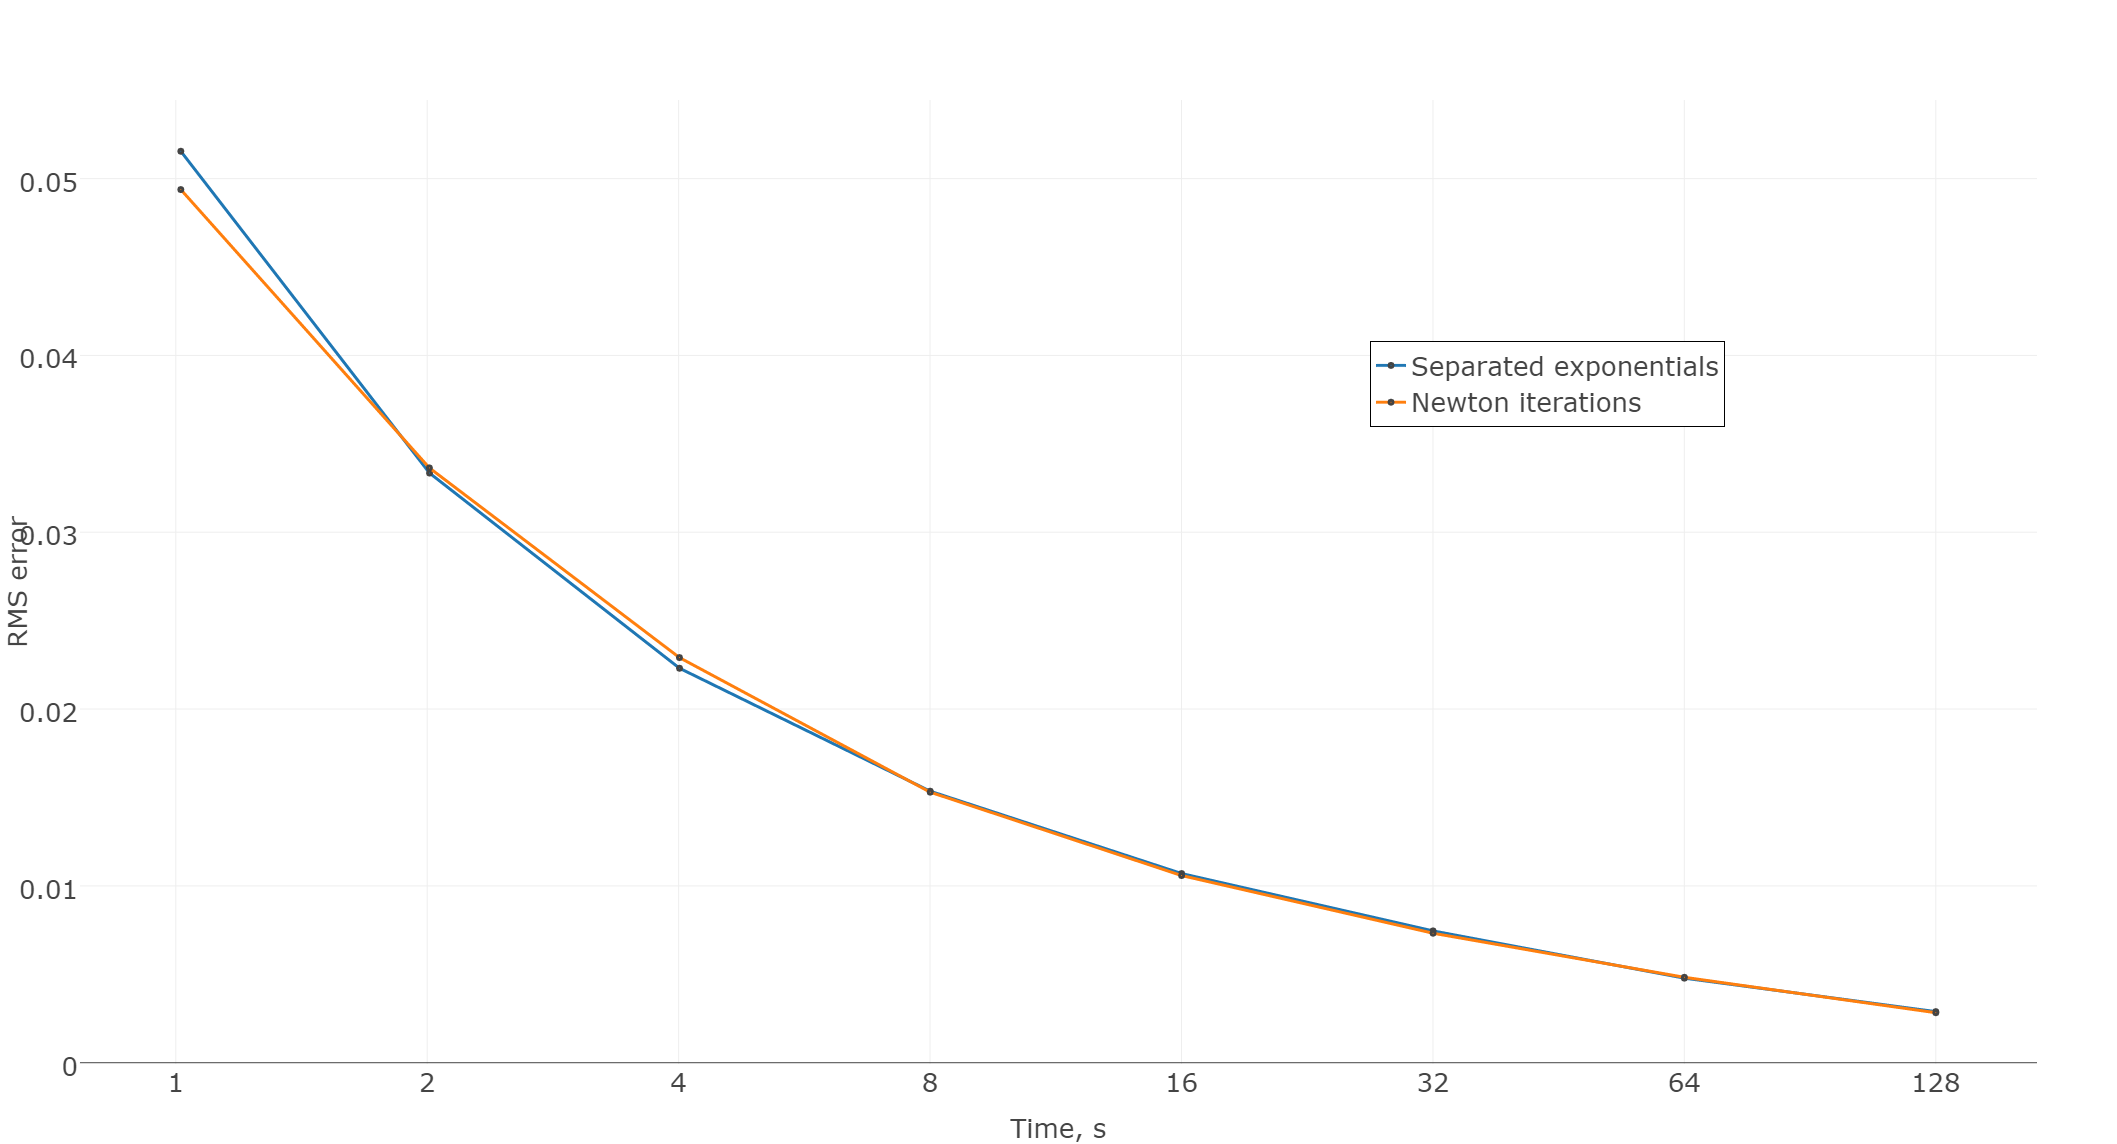
\includegraphics[width=\textwidth]{{imgs/plots/convergence_newton_exp}}
    \caption{Convergence plot over time of two importance sampling methods}
    \label{fig:importance_convergence}
\end{figure}

Both approaches result in almost identical convergence speed while measuring the error over the
whole image according to figure \ref{fig:importance_convergence}. In some cases Separated sampling
shows even better convergence. It can be observed while looking at the central part of the resulting
images after 5 seconds of rendering on figure \ref{fig:zoom_importance_sampling}.
\begin{figure}
    \centering
    \begin{subfigure}{0.3\textwidth}
        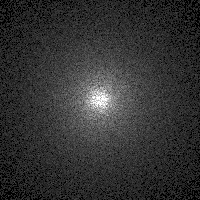
\includegraphics[width=\textwidth]{{{imgs/renders/cb_convergence/ref_exp_bigcrop_da_10.0_ds_0.1}}}
        \caption{Separated sampling}
        \label{fig:exponential_importance_sampling_zoom}
    \end{subfigure}
    \quad
    \begin{subfigure}{0.3\textwidth}
        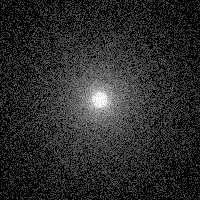
\includegraphics[width=\textwidth]{{{imgs/renders/cb_convergence/ref_newton_bigcrop_da_10.0_ds_0.1}}}
        \caption{Newton iteration}
        \label{fig:newton_importance_sampling_zoom}
    \end{subfigure}
    \caption{Equal time searchlight problem. Rendering results of the region close to the light
    source.}
    \label{fig:zoom_importance_sampling}
\end{figure}

But at the same time, this method produces unwanted fireflies in the regions far away from the light
incoming point. This effect can be seen at the figure \ref{fig:importance_sampling}. While
moderate intensity noise in the central region is reduced quite efficiently over time, the high
frequency spikes stay highly visible even after several minutes of rendering.

This is the reason why the Newton iteration was chosen as more robust and preferable importance
sampling technique for Christensen-Burley BSSRDF in out final implementation.
\begin{figure}
    \centering
    \begin{subfigure}{0.49\textwidth}
        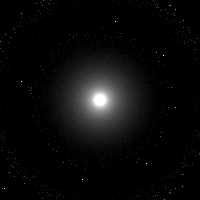
\includegraphics[width=\textwidth]{{{imgs/renders/cb_convergence/ref_exp_gamma_da_10.0_ds_0.1}}}
        \caption{Separated sampling}
        \label{fig:exponential_importance_sampling}
    \end{subfigure}
    \begin{subfigure}{0.49\textwidth}
        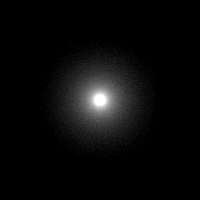
\includegraphics[width=\textwidth]{{{imgs/renders/cb_convergence/ref_newton_gamma_da_10.0_ds_0.1}}}
        \caption{Newton iteration}
        \label{fig:newton_importance_sampling}
    \end{subfigure}
    \caption{Equal time searchlight problem rendering comparison}
    \label{fig:importance_sampling}
\end{figure}

One of the possible solution of removing high frequency variance of the Separated importance
sampling is to clamp the high intense samples during rendering. This method, of course, introduces
additional bias to the final output and requires the control of the clamping threshold by the user.
But, taking into account the inherent biased nature of the Diffusion Approximation approach,
clamping may be a practical method of noise reduction with retaining lower variance in the region
close to the light.